\documentclass[]{article}
\usepackage{graphicx}
\usepackage{amsmath}
\usepackage{amssymb}
\usepackage{float}
\usepackage{hhline}

\graphicspath{ {./img/} }

\DeclareMathOperator*{\argmin}{arg\,min}

%opening
\title{Optim - HW2}
\author{Matteo Bunino}

\begin{document}

\maketitle


\section*{Problem 1}
\subsection*{Question 1 and 2}
Let $x\in R^m$, the function can be rewritten as:
\begin{equation}
	f(x) = (x-b)^TA(x-b)+3
\end{equation}
where $A$ ia diagonal matrix $A = diag(a_1, \dots, a_m)$.\\
The analytic forms of its gradient and its hessian are:
\begin{equation}
	\begin{aligned}
		& \nabla f(x) = 2A(x-b)\\
		& \nabla^2f(x)=2A
	\end{aligned}
\end{equation}
For the methods implementations, please refer to the function \textit{gradient\_descent} in the attached matlab code.\\
This function has two optional parameters \textit{alpha} and \textit{beta}: if they are specified, the gradient descent with backtracking will be performed. Otherwise, it will perform the gradient descent method with fixed step size.

\subsection*{Question 3}
Setting $a_i=1 \forall i$ means $A=I$, hence:
\begin{equation*}
	\nabla^2f(x)=2I\succeq2I \implies \text{$f(x)$ is strongly convex.}
\end{equation*}
Furthermore, the largest and the smallest eigenvalues are equal: $L=m=2$.\\
Hence, the rate of convergence of the method $O(\frac{L}{m}\log(\frac{1}{\epsilon}))$ becomes $O(\log(\frac{1}{\epsilon}))$.\\\\
The step size can be chosen as:
\begin{equation*}
	t\leq \frac{2}{L+m}
\end{equation*}
so I take $t=\frac{1}{2}$.\\\\
Since the objective is strongly convex, I can choose as a stopping criterion for the method
\begin{equation*}
	||\nabla f(x)||_2 \leq \sqrt{2m\epsilon}
\end{equation*}
for a given $\epsilon$ and $m=2$. \\
I decided to set $\epsilon = 10^{-16}$, which is sometimes referred to as \textit{machine precision} quantity.\\\\
To compare the two variants of the gradient method I plot the residuals $f(x^k) - f(x^*)$ against the number of iterations, which is possible since we know the close form of $f(x)$ and we know that it is strongly convex. Therefore, I can compute the minimum by solving the equation
\begin{equation}
	\begin{aligned}
		& \nabla f(x^*) = 0\\
		& 2A(x^*-b) = 0 \, \longleftrightarrow \, x^*=b
	\end{aligned}
\end{equation}
In this case, $b$ was chosen to have uniformly distributed components in $[0,100]$.\\\\
Since the matrix $A$ is well-conditioned (its conditioning number is 1), both methods converge rapidly. In particular, the gradient descent with fixed step size always converges in one iteration. On the other hand, the gradient method implementing backtracking may require few additional iterations sometimes.
\begin{figure}[H]
	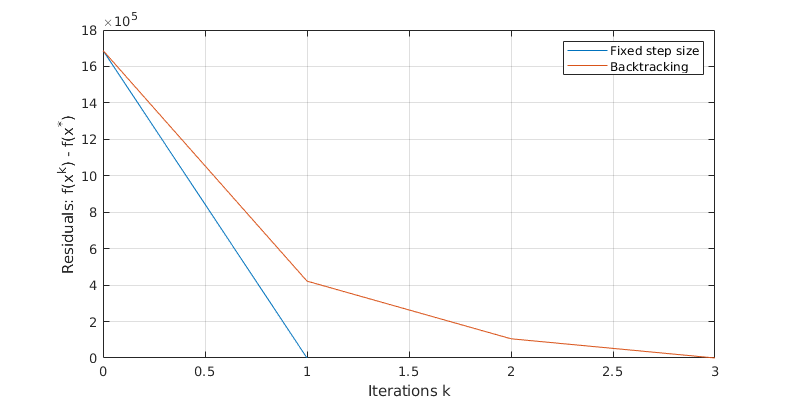
\includegraphics[scale=0.6]{1_3.png}
	\caption{Comparison between gradient method variants.}
\end{figure}


\subsection*{Question 4}
Now, I choose both $a_i$ and $b_i$ to be uniformly distributed components in $[1,100]$ $\forall i$, leaving all the other settings unchanged.\\
In matlab, I implement $A$ as a sparse matrix in order to save memory space and speed up the computations.\\\\
We can still prove that $f(x)$ is strongly convex, in fact:
\begin{equation*}
	\nabla^2f(x)=2I\succeq2I \implies \text{$f(x)$ is strongly convex.}
\end{equation*}
Hence, I set again the step as $t =\frac{2}{L+m}$ and I use the same stopping criterion based on the norm of the gradient of $f(x)$.\\\\
In this case, the conditioning number of $A$, which is the ratio of its largest and smallest eigenvalues $\frac{L}{m}$, is greater and can grow up to 100. This results in a slower convergence rate with respect to the previous case, which is $O(\frac{L}{m}\log(\frac{1}{\epsilon}))$ and can grow to  $O(100\log(\frac{1}{\epsilon}))$ in the worst case scenario.
\begin{figure}[H]
	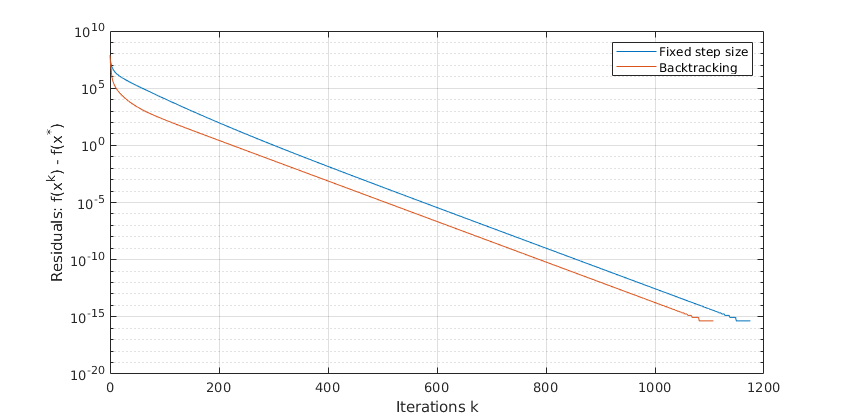
\includegraphics[scale=0.6]{1_4.png}
	\caption{Comparison between gradient method variants.}
	\label{1_4}
\end{figure}
As stated before, the convergence is slower due to the higher conditioning number of $A$. The graph reported in Figure \ref{1_4} was obtained with $A$ having a conditioning number of 98.008. Moreover, we can see the characteristic straight lines on semilog scale, underlying that the objective function is strongly convex.



\section*{Problem 2}
The optimization problem
\begin{subequations}
	\begin{alignat*}{2}
		&\!\min_{\mathbf{x}}        &\qquad& (\mathbf{x}-\mathbf{b})^TA(\mathbf{x}-\mathbf{b})+3\\
		&\text{subject to} &      & -\mathbf{x}\leq0,\\
		&                  &      & \mathbf{1}^T\mathbf{x} \leq 100.
	\end{alignat*}
\end{subequations}
can be rewritten as:
\begin{subequations}
	\begin{alignat*}{2}
		&\!\min_{\mathbf{x}}        &\qquad& (\mathbf{x}-\mathbf{b})^TA(\mathbf{x}-\mathbf{b})+3\\
		&\text{subject to} &      & C\mathbf{x}\leq \mathbf{d}.
	\end{alignat*}
\end{subequations}
where the two constraints have been rewritten in matrix form:
\[
C = \begin{bmatrix} 
	-1 & 0 & \dots  & 0\\
	0 & -1 &  & \vdots\\
	\vdots & & \ddots & 0\\
	0 & \dots & 0 & -1\\
	1 &  \dots & \dots     & 1 
\end{bmatrix}
\in R^{m+1 \times m}\] 
\[
d = \begin{bmatrix} 
	0 \\
	\vdots \\
	0\\
	100  
\end{bmatrix}
\in R^{m+1}
\]
and I recall that $A$ is a diagonal matrix $A=diag(a_1,\dots,a_m)$.\\\\
The corresponding Lagrangian function is:
\[
L(x,u) = (x-b)^TA(x-b)+3 + u^T(Cx-d)
\]
\subsection*{Question 1 - KKT conditions}
\subsubsection*{Stationarity}
\begin{equation}
	\label{stationarity}
	\frac{\partial}{\partial x}L(x,u) = 2A(x-b)+C^Tu = 0
\end{equation}
Solving for $x$:
\[
x^* = b-\frac{1}{2}A^{-1}C^Tu
\]
is the analytic form of the optimal solution $x^*$ of the problem, written as a function of the Lagrange multiplier $u$.
\subsubsection*{Complementary slackness}
The condition
\begin{equation}
	\label{complem}
	u_i\cdot h_i(x)=0, \forall i 
	\,\, \longleftrightarrow \,\,
	u_i\cdot (Cx-d)_i=0, \forall i 
\end{equation}
means that when $h_i(x) < 0$, the corresponding component $u_i$ of the Lagrange multiplier should be 0 because the constrain is not currently \textit{active}.\\
Otherwise, if $x$ is on the boundary of the feasible set the constraint $h_i(x)$ is active and can be rewritten as an equality constraint $h_i(x) =0$. 
Hence, Equation \ref{complem} is verified for each $i$.\\
Based on these observations there exist a class of optimization algorithms called \textit{Active set methods}.\\\\
Let $U=diag(u)$, this condition can be rewritten in matrix form as:
\[ U(Cx-d) = 0 \]

\subsubsection*{Primal feasibility}
\[ Cx-d \leq 0\]
This condition is required in the formulation of the primal problem.

\subsubsection*{Dual feasibility}
\[ u\geq0 \]
This condition is required because we want to penalize a violation of the inequality constraints of the primal problem in the Lagrangian function.\\
In other words, if $u_i<0$ for some $i$, minimizing $L(x,u)$ over $x$ would give a solution such that $h_i(x)>0$ for some $i$.

\subsection*{Question 2 - Dual Problem}
From the stationarity condition, by solving Equation \ref{stationarity}, I obtain the analytic formula for the optimal $x^*$ as a function of the Lagrange multiplayer $u$, when $u\geq0$.
\[
x^* = \argmin_x L(x,u) =  b-\frac{1}{2}A^{-1}C^Tu
\]
The Lagrange dual function is:
\begin{equation*}
	\begin{aligned}
		g(u) &= L(x^*,u)\\
		&=\dots \text{(I skip all the steps).}\\
		&= -\frac{1}{2}u^TCA^{-1}C^Tu+u^T(Cb-d)+3 
	\end{aligned}
\end{equation*}
and the corresponding dual problem is:
\begin{subequations}
	\begin{alignat*}{2}
		&\!\max_{\mathbf{u}} &\qquad& -\frac{1}{2}\mathbf{u}^TCA^{-1}C^T\mathbf{u}+\mathbf{u}^T(C\mathbf{b}-\mathbf{d})+3\\
		&\text{subject to} & & \mathbf{u}\geq 0.
	\end{alignat*}
\end{subequations}
The gradient and the hessian of $g(u)$ are:
\begin{equation*}
	\begin{aligned}
		& \nabla g(u) = -CA^{-1}C^T\mathbf{u}+C\mathbf{b}-\mathbf{d}\\
		& \nabla^2 g(u) =-CA^{-1}C^T
	\end{aligned}
\end{equation*}
I can do the following observations on the Lagrangian dual function:
\begin{itemize}
	\item From theory we know that the Lagrangian dual function is always \textbf{concave} because it it the infimum of $L(x,u)$, which is an affine function in $u$.\\
	For this reason, I can alternatively say that $\phi(u) = -g(u)$ is convex and has $\nabla \phi(u) = -\nabla g(u)$ and $\nabla^2 \phi(u) = -\nabla^2 g(u)$.
	\item Recalling that $A$ is a symmetric matrix, we can easily prove that $ \nabla^2 g(u)$ and $\nabla^2 \phi(u)$ are symmetric, hence all of their eigenvalues are real.\\
	Hence, we can prove that $-g(u)$ is Lipschitz continuous and there exists a constant $L>0$ such that $-\nabla^2 g(u) \preceq LI$.
	\item However, we cannot prove that $-\nabla^2 g(u)$ is positive definite, hence:\\
	$\nexists m>0: -\nabla^2 g(u) \succeq mI$. Therefore, I cannot exploit anymore the properties of strong convexity for $\phi(u)$ (or strong concavity in the case of $g(u)$).
\end{itemize}
Since the constrain is simple (nonnegative orthant), I can solve this problem by performing the projected gradient ascent method, or alternatively, the projected gradient descent on $\phi(u) = -g(u)$.\\\\
Since $\phi(u)$ is convex but not strongly convex, I can take a step size $t \leq \frac{1}{L}$, hence I take $t = \frac{1}{L}$.\\\\
The projected gradient descent is a proximal method and it requires a number of iterations $O(\frac{1}{\epsilon})$ to find a $\epsilon$-suboptimal point.\\\\
Since the problem is constrained, I cannot set a stopping criterion based on the norm of the gradient, because the gradient in the optimal point could not attain a zero norm. For this reason I take a sufficiently small $\gamma$ and I stop the method 
\[
||u^k-u^{k-1}||_2 < \gamma
\]
Namely, I assume the method to have converged when the Euclidean distance between the last two $u^k$ is lower than a given threshold $\gamma$.\\
I also set the maximum number of iterations to be equal to $\frac{1}{\epsilon}$.\\
After some tuning, I set $\gamma=1e{-8}$ and $\epsilon=1e{-8}$.\\\\
I solve the problem where $m=500$ and  both $a_i$ and $b_i$ to be uniformly distributed components in $[1,100]$ $\forall i$.\\
Since $A$, $C$ and $d$ are pretty sparse, I implement them in matlab as sparse matrices, in order to save memory space and speed up the matrix operations.\\
The implementation of the projected gradient descent method over $\phi(u)$ can be found in the attached matlab code, as the function \textit{proj\_gradient\_descent}.\\\\
\textbf{Convergence analysis}
\begin{figure}[H]
	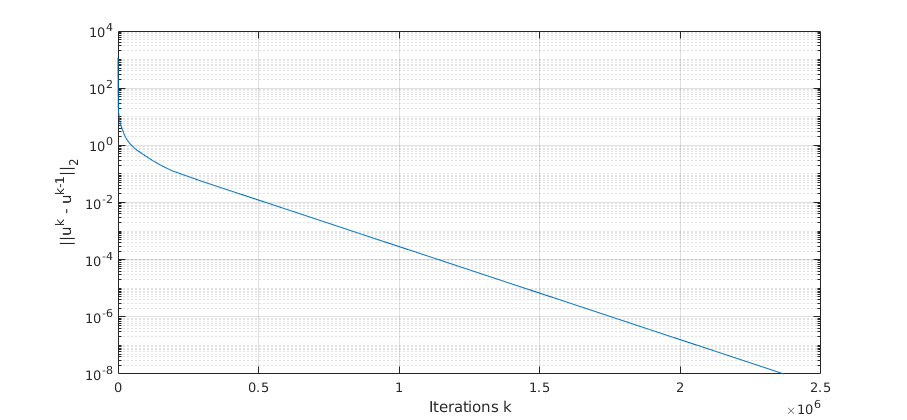
\includegraphics[scale=0.55]{2_2.png}
	\caption{Dual projected gradient ascent with fixed step size.}
	\label{2_2}
\end{figure}
As stated before, $g(u)$ ($\phi(u)$) is not strongly concave (convex), hence the semilogy plot of  $||u^k-u^{k-1}||_2$ against the number of iterations is not a perfect line.\\\\
To check the feasibility of the attained solution $x^*$ i perform the following two matlab commands:
\begin{itemize}
	\item sum(x\_star): has to be $\leq$ 100.
	\item sum(x\_star<-1e-7): has to be 0. I use the negative threshold -1e-7 because I am working up to a tolerance 1e-8 on $u^*$ and there may also be numerical cancellation effects, hence I cannot ask for an exact solution. Hence I ask $x$ being non-negative, up to a tolerance of 1e-7.
\end{itemize}


\subsection*{Question 3 - Parallelization}
The optimization problem can indeed be parallelized because it can be rewritten as a sum of $m$ independent functions, each one taking a scalar $x_i$.\\
This problem can be parallelized on up to $m$ nodes, each one solving the problem
\begin{subequations}
	\begin{alignat*}{2}
		&\!\min_{x_i} &\qquad& f_i(x_i) = a_i(x_i-b_i)^2\\
		&\text{subject to} &      & x_i\geq0,\\
		&&&  \mathbf{1}^T\mathbf{x} \leq 100.
	\end{alignat*}
\end{subequations}
However, we have to guarantee that the last constraint is shared among all the nodes, which unfortunately has an impact on the performances.\\
In fact, at each iteration all the nodes should share their local $x_i$ with the others in order to guarantee that the final solution will be a feasible $x*$. This communication cost depends on the topology of the network that connects all the nodes: the more connected is the network, the higher is the impact of network communication delays, but the faster is the overall convergence of the method.\\
For instance, if we implement a clique network, we can achieve the fastest information propagation among nodes.\\
Eventually, if the network topology is well designed, parallelization can improve the overall convergence speed even though the total number of iterations are the same as the method without parallelization. This is a way to distribute the load among different nodes.\\


\end{document}
